\section{Security and Deniability}
\label{sec:dis_sec}
The data stored in \gls{FFS} images is encrypted with \mbox{state-of-the-art} encryption standards. Using \gls{AES}-\gls{GCM}, \gls{FFS} not only provides confidentiality of the data, but it also provides the authenticity of the data. The cryptographic algorithms are implemented using good cryptographic standards, such as cryptographic secure number generators\,\cite{RandomNumberGeneratorCryptoWiki2021}. However, the security of \gls{FFS} is dependent on, among other things, the password the user chooses. A bad password, for instance, short or commonly used, is easily breakable for an adversary. An adversary who has access to an \gls{FFS} encrypted image could \mbox{brute-force} the bad password used to derive the encryption key much faster than they could \mbox{brute-force} the decryption key. \gls{FFS} does not put any constraints on the password used - as long as it is at least one byte it is acceptable for \gls{FFS}. This puts the responsibility on the user for a secure password. 

\gls{FFS} puts a lot of trust in the \mbox{open-source} library Crypto++\,\cite{CryptoLibraryFree}. Crypto++ provides cryptographic functions that \gls{FFS} uses for, among other things, deriving the encryption key, encrypting the data, and verifying the authentication tag. While there are no reported CVE security vulnerabilities as of the time of this writing\,\cite{CryptoppSecurityVulnerabilities}, there may be vulnerabilities that have not yet been discovered or that have been found but not published in the CVE database. There is also a possibility that \gls{FFS} has vulnerabilities, such as side channels, which could be exploited. \gls{FFS} was developed by a single author without a review from anyone.

Anyone with access to Flickr.com can view and download the original images stored by \gls{FFS}, both registered users on Flickr, and anonymous visitors, even if the uploader has restricted access to their originally uploaded images\,\cite{FlickrHelpForum2020}. An example of how the profile might look is shown in Figure~\ref{fig:flickr_profile}. The images found on the account present little information about the filesystem. For users unaware of \gls{FFS} who view the Flickr profile, they see different sizes of images with seemingly randomly generated pixel colors. However, for adversaries who know about the details of \gls{FFS}, more information can be retrieved. For instance, they could assume that the most recently uploaded image to Flickr is the inode table. However, as we assume the adversary does not have access to the decryption key, they cannot decode the \mbox{plain-text} data of the image and thus cannot verify that this is indeed the inode table. The exact number of files and directories in \gls{FFS} cannot be known precisely without access to the content of the inode table. Even if the Flickr account has, for instance, 15 images stored, and we know that one represents the inode table and one represents the root directory, it is not possible to conclude if other images stores file data or directory data. The remaining 13 images in the example could represent:
\needspace{7\baselineskip}
\begin{itemize}
	\item one big single file split over 13 images, or
	\item one big single directory split over 13 images, or
	\item 13 different files, or
	\item 13 different directories, or
	\item one directory and 12 different files, or
	\item 13 copies of the same file, et cetera.
\end{itemize}
It is possible to see the size of an image, and a big image can suggest that a file or directory consists of multiple images on Flickr.

It is also not possible to know if an image stored on Flickr has been uploaded by \gls{FFS} or by the user manually to further inflate and diffuse the amount of data stored on the service. For instance, by encrypting random data using \gls{FFS}'s encoder and uploading the images to Flickr, but without saving the posts in the inode table or in a directory of \gls{FFS}, the images will look indistinguishable from the other images on Flickr. Only with access to the decrypted inode table can one know if the image is relevant to \gls{FFS} or not. However, it is possible that Flickr could have logs about the uploaded images, and can be able to distinguish images uploaded from the \gls{API} from the user interface. Future research could extend \gls{FFS} to post encrypted random data at random time intervals to automatically diffuse the knowledge about the images on the \gls{OWS}. This would mean that even Flickr would be unable to distinguish the uploaded data as it would all be uploaded from the same service. \gls{FFS} would be required to upload the diffusing data using the same pattern as is used when a file or directory is updated or created so that the upload pattern for the diffusing data is undistinguishable from the regular data for users without the decryption keys. For instance, a write operation on a file will remove the old file and the old inode table, and upload one new image as the new file data and one new image as the new inode table. Similarly, for a new file created in the filesystem, the new file content is uploaded as an image, one image is uploaded as the parent directory's new data, one image is uploaded as the new inode table, and the old directory image and inode table image are removed from Flickr. To simulate file write and file create filesystem operations, two or three images must be uploaded and two images must be deleted. One problem with this could be that the last image uploaded should always be the inode table. While the data of the inode table can easily change by changing the encryption key, the size of the inode table could remain the same which could be suspicious for adversaries with access to snapshots of the Flickr account's images. This could be solved by always adding a random amount of filler bytes when encoding the image. The filler bytes are not read by the decoder anyway. However, adding filler bytes can increase the resulting file size of the images, decreasing the overall storage capacity of \gls{FFS}. Furthermore, storing diffusing images on Flickr that are not stored in the \gls{FFS} filesystem decreases the storage capacity of \gls{FFS}.

\begin{figure}[!h]
	\begin{center}
	  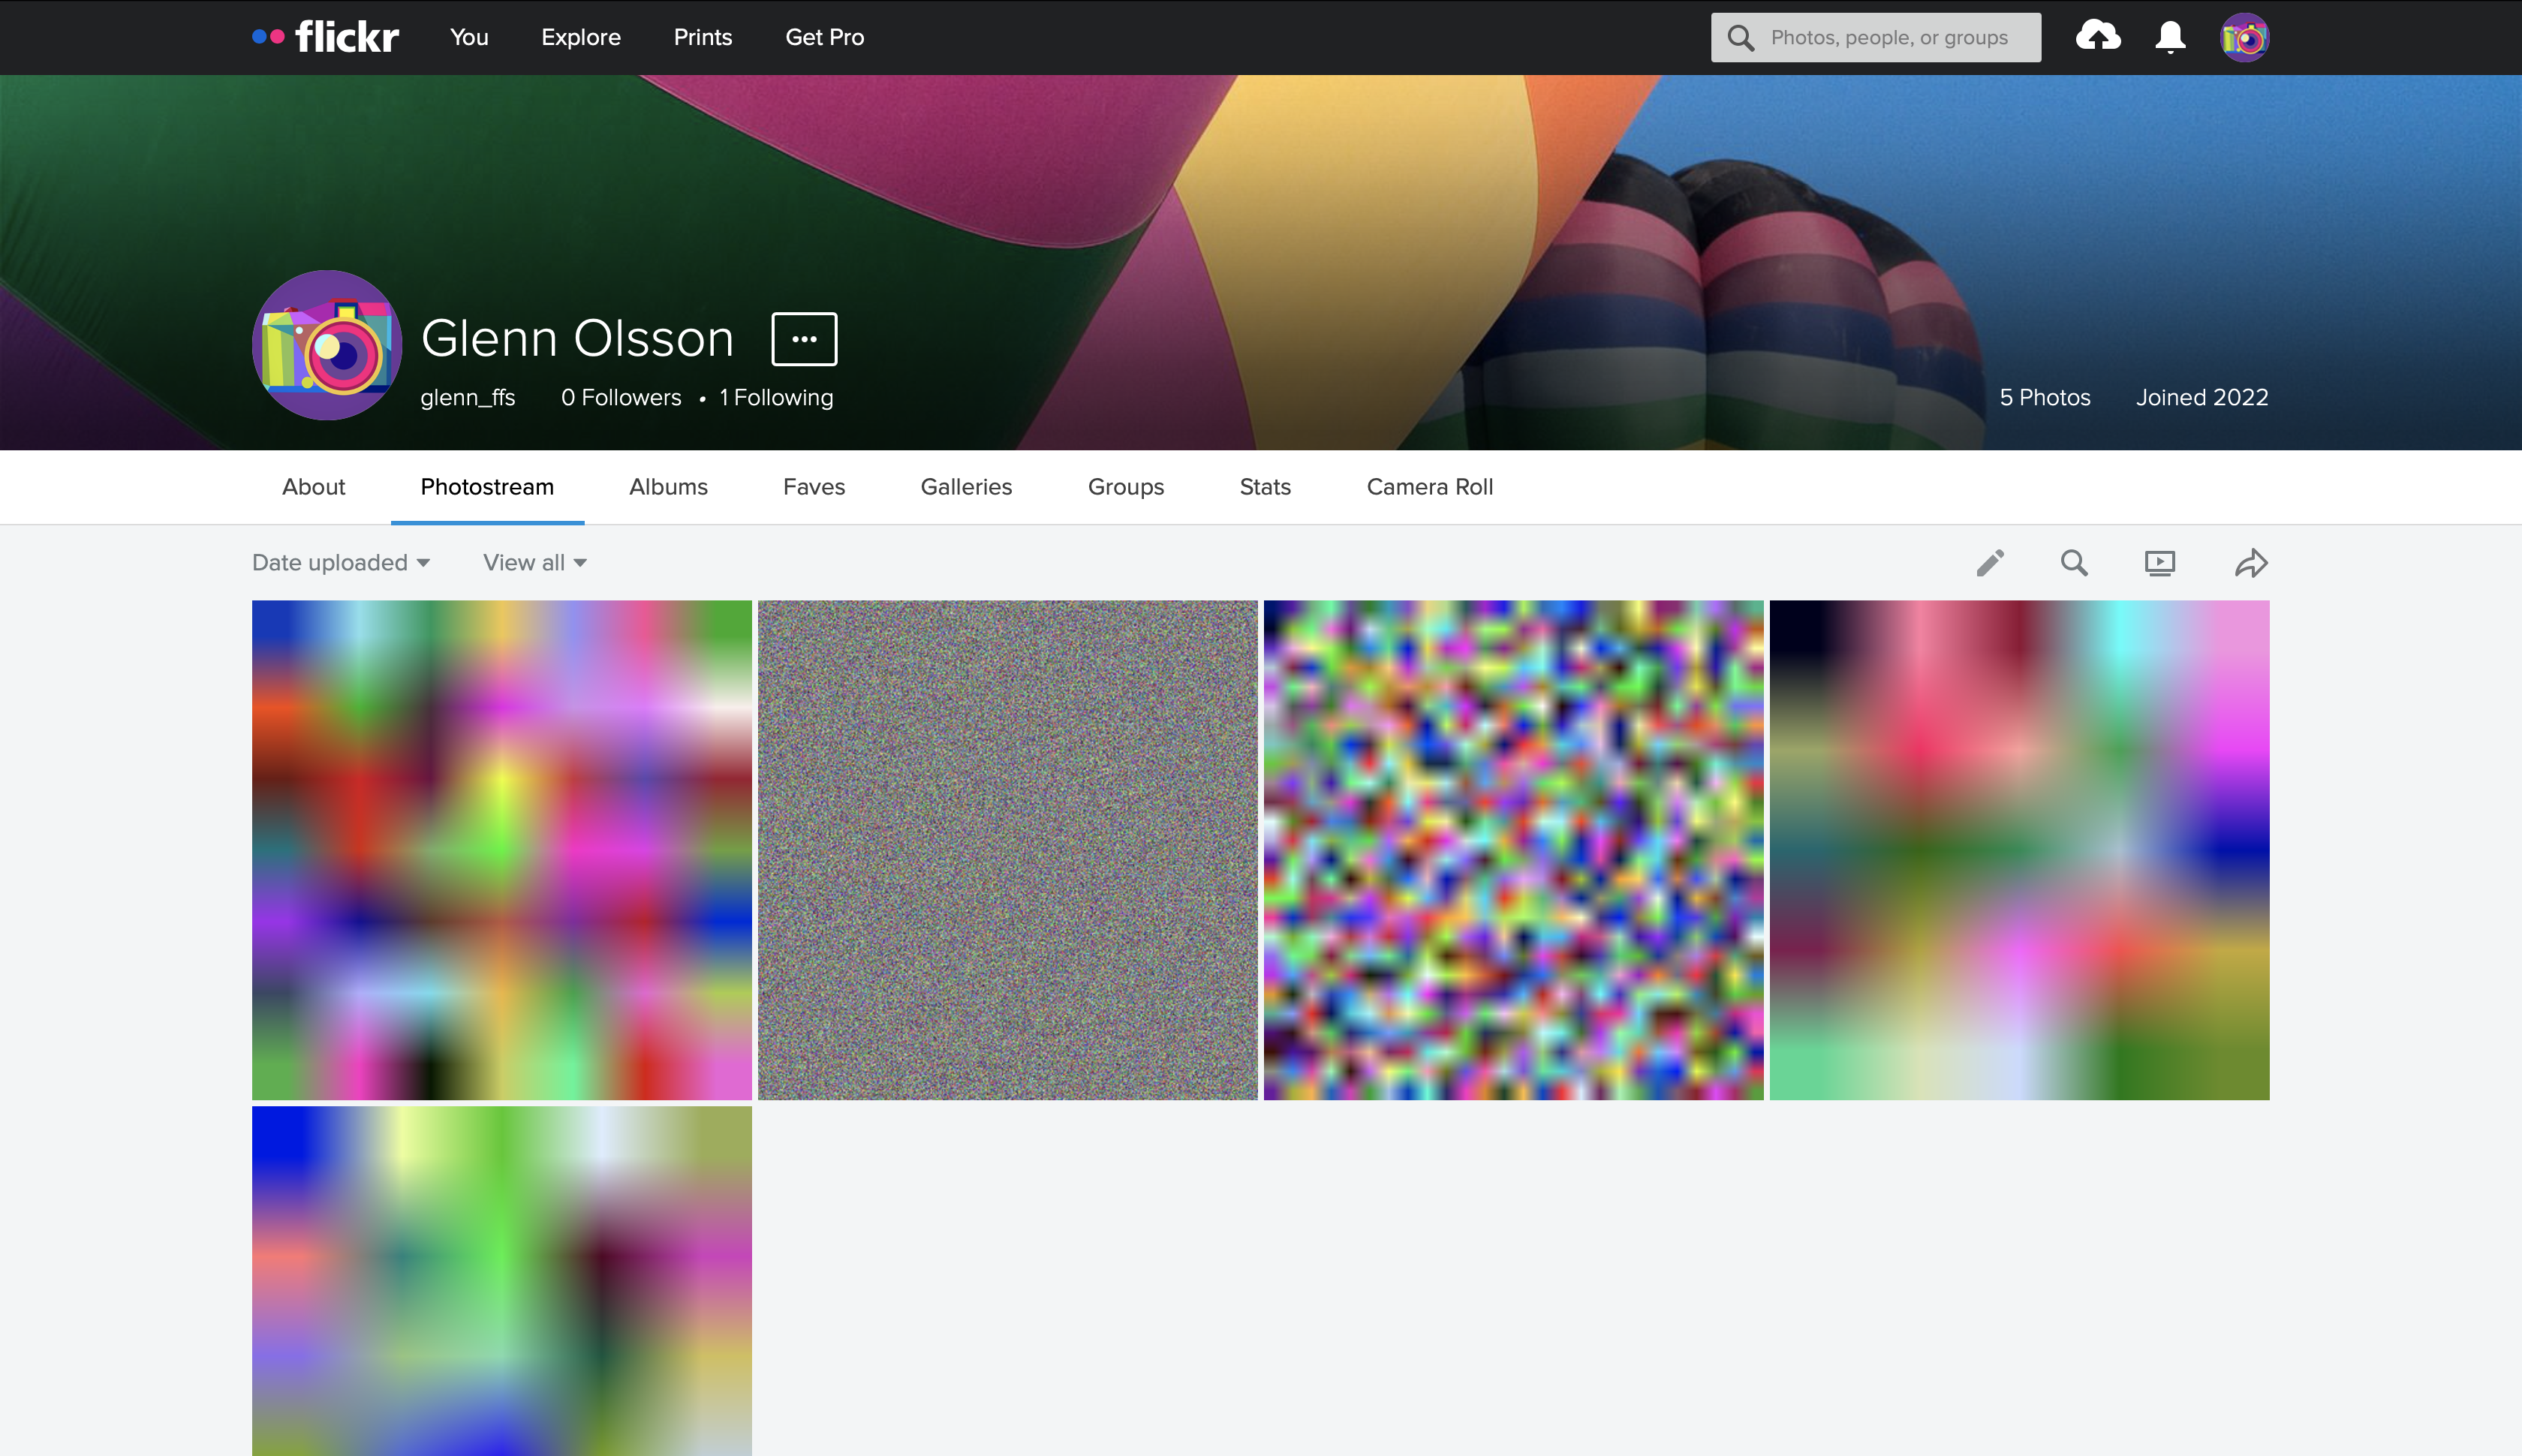
\includegraphics[width=0.8\textwidth]{figures/flickr_profile.png}
	\end{center}
	\caption[Screenshot of the Flickr profile used for \gls{FFS}]{Screenshot of the Flickr profile used for \gls{FFS}. At the moment of the screenshot, the filesystem is storing a previous version of this thesis in a directory inside the root directory. The images seen are the inode table, the thesis data, the root directory data, the subdirectory (containing the thesis) data, and a temporary file containing extra attributes of the thesis document created by macOS while \gls{FFS} was mounted (this file is sometimes referred to as a \textit{turd}\,\cite{geekosaurAnswerWhyAre2011}).}
	\label{fig:flickr_profile}
\end{figure}

The size of data stored in an image is not completely hidden. While the exact number of bytes of unencrypted data that the image stored is not possible to know without the decryption key, it is possible to get an estimate. If you know the binary structure of the image (as presented in Appendix~\ref{app:binary_rep}), you can find out how many bytes the encrypted cipher is, the value of the \gls{IV} data, the value of the salt used for the encryption key derivation, and the value of the authentication tag. By knowing the length of the cipher, the length of the unencrypted data can be placed in a range. The length of the cipher $L_c$ in bytes is divisible by 16 (as \gls{AES} is a \mbox{16-byte} block cipher), and the length of the plain text must be less than $L_c$ due to the requirement of at least one bit of padding\,\cite{z.z.coderAnswerSizeData2010}. The smallest possible size for the length of the plain text is $L_c - 16$. Therefore, the length of the plain text $L_p$ is:
$$
	L_c - 16 \leq L_p < L_c
$$
By examining all the images stored on Flickr and the possible values of $L_p$, it is possible to know the upper limit and lower limit of all the \gls{FFS} data stored on Flickr at a certain time, assuming that all images on Flickr are stored in \gls{FFS}. However, it is \textbf{not} possible to know if all this data is stored on \gls{FFS} through entries in the inode table. It is also \textbf{not} possible to know if the plain text represents a file or directory without the decrypted data of the inode table. One image can be assumed to be the inode table of which a \mbox{size-estimate} is also possible. 

If a user supplies a different password when mounting \gls{FFS} than used previously, the images stored on Flickr cannot be decrypted. When \gls{FFS} tries to read the image it believes represents the inode table (the most recently uploaded image) and it fails, it will simply create a new inode table representing an empty filesystem, and upload the image representing this inode table, essentially replacing the potentially previous inode table (if it existed). As it is not possible to know if the images already uploaded to Flickr represent an inode table without the correct decryption key, it is impossible to determine if the image that could represent the inode table is indeed an inode table encrypted with another password, or if it is some arbitrary data. In a potential \mbox{rubber-hose} situation\footnote{When an adversary might torture the user, with for instance a rubber hose. See Section~\ref{sec:rubber_hose}}, the user of the filesystem could easily claim that they uploaded \gls{FFS} images with arbitrary data, using randomly generated keys that they do not remember and that the filesystem is empty. There is no way to prove the existence of any meaningful data on Flickr without the decryption key. As the \gls{FFS} encoder also uses random salting for the encryption key, it is not even possible to prove that the images are encrypted with the same password as the encryption keys will differ for all images, even when the same password is used. 

However, as mentioned earlier, we assume that an adversary has access to the structure of \gls{FFS} images as well. To counter this, the user who want to hide their data could, after creating a filesystem containing meaningful information, mount \gls{FFS} again with another password. \gls{FFS} would then create a new inode table and upload this table, creating a dummy \gls{FFS}. In a \mbox{rubber-hose} situation, the user could give up the password to the dummy \gls{FFS} instance, which is empty. The adversary can verify that this password indeed decrypts the most recently uploaded image and that the unencrypted image data represents an empty inode table. If the user proceeds to claim that they do not know the passwords of the other images, the adversary cannot prove that they contain meaningful data or that they have been uploaded by the user. These images could, for instance, have been uploaded by another user of \gls{FFS}. Further, with no password constraints by \gls{FFS}, a user could also create a dummy \gls{FFS} with a password that is easily breakable, to make the adversary believe they found the correct password if they perform a \mbox{brute-force} attack. As long as the user remembers which post represents the inode table, the images uploaded after this inode table could simply be removed from Flickr before mounting \gls{FFS} with the correct password when the user want to access their actual \gls{FFS} instance. Alternatively, the user could save the image representing the inode table in another storage medium and upload it again when they want to access their actual \gls{FFS} instance.

One aspect where \gls{FFS} is better than \gls{GCSF} is its security against the potential adversary of the storage owners. \gls{GCSF} stores the data in its original format on Google Drive, essentially providing an overlay filesystem for Google Drive. While this can be desired in certain situations, such as using \gls{GCSF} on one machine and the Google Drive website on another, it gives Google Drive access to your data. As mentioned, Google Drive encrypts your data from outside agents, but as they control the encryption and decryption keys themselves, the data stored can be accessed by the company. The data could also be given to authorities who are requesting it with a subpoena. However, to use Google Drive while maintaining your own encryption methods, an overlay filesystem could be mounted on top of \gls{GCSF} using a stackable filesystem, such as Cryptfs\,\cite{zadokCryptfsStackableVnode1998}. Future work could include researching the performance of such an overlay filesystem on \gls{GCSF} and compare it to \gls{FFS}.

\gls{FFS} on the other hand gives the user control of all its data. While Flickr can give out the images uploaded by \gls{FFS}, this data can be accessed by anyone with access to Flickr.com anyway. The only way to access unencrypted data is by using the password that the user controls. This provides \gls{FFS} with one aspect of better security than \gls{GCSF}, but this might also be a factor why \gls{FFS} is slower than \gls{GCSF}. By requiring the data to be encrypted when it is written and uploaded, and decrypted when it is downloaded and read, \gls{FFS} will need to compute new cryptographic variables every time a file or directory is written which requires a lot of computations. Further, every time an image is read it must be decrypted, even if it is in the cache of \gls{FFS}. Decrypting an image requires a lot of computations as well, as other than decrypting the data, the decryption key must first be derived from the password. Meanwhile, it is possible that Google Drive is caching the unencrypted files, or performing the cryptographic computations on \mbox{high-performance} computers requiring less computation time. So while gaining a security aspect of the filesystem, \gls{FFS} sacrifices the performance of the filesystem operations.

Every \gls{ISP} in Sweden is required to keep data generated or managed during internet access for ten months\,\cite{post-ochtelestyrelsenFragorOchSvar2019}. \gls{ECJ} has declared that retained data should only be accessed when fighting serious crimes or if national security is at stake\,\cite{EuropeanCourtJustice2017}. In the United States, there are no data retention laws requiring \gls{ISP}s to store identifiable information, however, no major American \gls{ISP} has enacted zero data retention policies\,\cite{lawofficesofsalaratrizadehUnitedStatesData2021}. Furthermore, American \gls{ISP}s can be forced to give out what information they have about a customer by US law, including the websites the customer has been visiting\,\cite{instituteDataRetentionLaws}. Using \gls{FFS} or \gls{GCSF}, your \gls{ISP} can identify your internet traffic and know that you are accessing Flickr or Google Drive. Furthermore, by combining the data with the IP logs of Flickr or Google Drive, it could also be possible to identify you as the uploader of data to \gls{FFS} or \gls{GCSF}. However, technologies such as Tor or a \gls{VPN} could hide your identity from your \gls{ISP}. According to Swedish law, \gls{VPN} providers are not required to retain logs of its users\,\cite{walshInternetCensorshipSweden2020}. However, they are not prohibited from storing such data. Furthermore, the \gls{ISP} of the \gls{VPN} provider must still log the network traffic originating from the \gls{VPN} service. Even though they cannot identify specific users without logs from the \gls{VPN} provider, they can determine what websites are accessed from the \gls{VPN} service, even though they might not know that the service is a \gls{VPN} provider. If the \gls{VPN} provides logs about you to adversaries, you could still be identified. Tor provides the user with multiple routing layers to hide the origin of the internet traffic\,\cite{ramadhaniAnonymityCommunicationVPN2018}. The internet connection is encrypted and the source IP address is changed for each hop, and the final node has no information about the original source address of the request. Furthermore, the nodes used by the client are changed periodically. However, Tor is slow due to the layered connections and would therefore decrease the already low performance of \gls{FFS} further. 

\gls{FFS} writes temporary files to the local filesystem when uploading images to Flickr due to limitations in the Flickr library used. Even though the images are stored for a short time in the filesystem and removed shortly after being created, there are possibilities to recover removed data from \gls{APFS}\,\cite{llcsysdevlaboratoriesHowRecoverData2022,cedricAPFSDataRecovery2022,santosHowRecoverData2021}. Furthermore, if \gls{FFS} would crash for some reason while uploading a file, the temporary file could remain readable in the \gls{APFS} filesystem. This could be solved by storing the temporary file in a temporary filesystem. For instance, a secure in-memory \gls{FUSE} filesystem could be mounted on the computer and be used as the temporary file storage. This is part of future work for \gls{FFS}.

Flickr state in their community guidelines\,\cite{flickrinc.FlickrCommunityGuidelines2022} that they do not allow non-photographic elements in their service. \gls{FFS} uploads images with seemingly random noise, not photographs. It is therefore probable that Flickr would remove the images uploaded by \gls{FFS} if they were discovered or reported by the community. Another adversary of \gls{FFS} is thus detection from Flickr. During testing of the filesystem, while big files have been uploaded, there have not been more than 50 images stored on Flickr by \gls{FFS} at a time which is far from their $1\,000$ image limit. No \gls{FFS} images has been removed from Flicker as of writing and it is possible that the Flickr account has not raised suspicion from Flickr due to the low number of images. If images were removed from Flickr, it could have very negative effects on the usability of the filesystem. For instance, if the image representing the inode table was removed, the post ID of each filesystem would be lost unless \gls{FFS} was running at the same time as the inode table is cached in memory. While the images could still be decrypted by \gls{FFS}, the filename and path of each file and directory would be lost. If an image representing a directory was removed (but the inode table was not removed), the files and directories in the directory would not have a filename associated with them. They would also not be findable in the filesystem as \gls{FFS} does not support links, so there is only one filepath per file or directory in the filesystem. If an image representing a file was removed, the file data would be lost. If an image representing one part of a file was removed, only the data stored in that image would be lost. The remaining images could still be decoded and decrypted on their own, but the lost data cannot be recovered. It is important that the images are not removed from the \gls{OWS} for the data stored in \gls{FFS} to be safe. However, this guarantee is hard to achieve as the Flickr terms of service state that Flickr retains the right to remove user content from the service at any time\,\cite{flickrinc.FlickrTermsConditions2020}. If Flickr would have knowledge about \gls{FFS} it is possible that they would implement detection techniques of the \gls{FFS} images, and remove them. Combating detection by the \gls{OWS} is part of future work.

% timestamp: 
% - Can see when image was uploaded
% - Can see when ffs was written to/modified
% - Basically a log of when FFS was accessed by the user
% - Could find out the origin of the upload using ISP data?
% - Part of paragraph above?
% TODO: 
%	- Exploit possibilities of saving the Inode table last? "This would seem to mean that one can exploit the dates of this image to know when the FFS was last written to. By correlating this with network accesses the identity and locations of the user can be inferred."